\documentclass[a4paper,12pt]{article}
\usepackage{graphicx}
\usepackage{amsmath}
\usepackage{hyperref}
\usepackage{geometry}
\usepackage{algorithm}
\usepackage{algorithmic}
\usepackage{listings}
\usepackage{url}

\geometry{margin=1in}

\title{Evaluation of Privacy-Preserving Machine Learning with Fully Homomorphic Encryption (FHE)}
\author{ Licciardi Oscar}

\date{\today}

\begin{document}

\maketitle

\section*{Abstract}
This study presents a comprehensive evaluation of privacy-preserving machine learning using Fully Homomorphic Encryption (FHE). We compare plaintext models implemented with scikit-learn to ciphertext models trained with Concrete-ML across multiple dimensions. Our analysis focuses on metrics such as accuracy, latency, and the impact of bit-width on model performance to understand the trade-offs involved in using FHE for machine learning tasks. Key findings show that FHE models can achieve comparable accuracy to plaintext models (up to 99.85\% for Logistic Regression), though with varying computational overhead (5.15× for Decision Trees, 6.13× for Logistic Regression, and 46.79× for Random Forest). We also discovered that optimal bit-width is highly model-dependent, with lower bit-widths sometimes yielding better accuracy while reducing computational demands. These results demonstrate that privacy-preserving machine learning with FHE is becoming increasingly viable for practical applications, especially for models with simpler computational structures. Our proposed evaluation framework provides a systematic approach for assessing the performance-privacy trade-offs when implementing privacy-preserving machine learning systems.

\section{Introduction}
Privacy-preserving machine learning has gained significant attention due to the increasing need to process sensitive data securely while maintaining compliance with stringent data protection regulations such as GDPR, HIPAA, and CCPA. Traditional machine learning approaches require access to raw data during both training and inference phases, creating potential vulnerabilities for data breaches and unauthorized access. This challenge is particularly acute in domains like healthcare, finance, and personal identity information, where data is both highly sensitive and valuable for building predictive models.

Fully Homomorphic Encryption (FHE) offers a promising solution to this dilemma by enabling computations directly on encrypted data without requiring decryption. In theory, this approach allows machine learning models to make predictions on sensitive data without ever exposing the underlying information, thereby maintaining privacy throughout the entire process. However, FHE operations are computationally intensive, potentially introducing significant performance overhead and raising questions about their practicality in real-world applications.

The fundamental research question driving this study is: To what extent can FHE-based machine learning provide privacy guarantees while maintaining competitive performance in terms of accuracy and computational efficiency? More specifically, we aim to answer:

\begin{itemize}
    \item What is the accuracy trade-off when transitioning from plaintext to FHE-based machine learning models?
    \item How significant is the computational overhead introduced by FHE operations across different model architectures?
    \item What is the impact of precision (bit-width) on both accuracy and latency in FHE models?
    \item Which model architectures are most suitable for privacy-preserving applications using FHE?
\end{itemize}

This research aims to:
\begin{itemize}
    \item Compare the performance of plaintext models (scikit-learn) and ciphertext models (Concrete-ML) across multiple metrics.
    \item Analyze the impact of bit-width on accuracy and latency for ciphertext models to determine optimal configurations.
    \item Develop a systematic evaluation framework for assessing FHE-based machine learning models.
    \item Identify areas for further investigation, such as the scalability of FHE models to larger datasets and the impact of different encryption schemes on model performance.
\end{itemize}

The significance of this work lies in its practical contribution to the field of privacy-preserving machine learning. By quantifying the trade-offs involved in implementing FHE for machine learning tasks, we provide practitioners with actionable insights for designing secure machine learning systems that protect sensitive data without sacrificing performance. This research also contributes to the growing body of literature on practical applications of homomorphic encryption, helping bridge the gap between theoretical advances and real-world implementations.

\section{Methodology}

\subsection{Dataset}
We used a credit card fraud detection dataset containing 284,807 transactions, of which 492 (0.17\%) were fraudulent. This highly imbalanced dataset represents a challenging but realistic scenario for privacy-preserving machine learning applications. The dataset was preprocessed and split into training (80\%) and testing (20\%) sets.

\subsection{Model Implementation}

\subsubsection{Plaintext Models}
Plaintext models were implemented using scikit-learn with hyperparameter optimization through grid search. The following configurations were identified as optimal:

\begin{itemize}
    \item \textbf{Logistic Regression}: C=0.1, penalty='l2', solver='liblinear'
    \item \textbf{Random Forest}: max\_depth=7, min\_samples\_leaf=3, n\_estimators=100
    \item \textbf{Decision Tree}: max\_depth=3, min\_samples\_leaf=4, min\_samples\_split=2
\end{itemize}

\subsection{FHE Models}
FHE models were implemented using Concrete-ML \cite{concrete-ml}, which provides a framework for privacy-preserving machine learning with FHE. Models were trained on plaintext data and optimized for inference on encrypted data. We evaluated multiple bit-width configurations (2, 3, 4, 6, and 8 bits) to understand the impact of precision on model performance.

\section{Concrete-ML Library Overview}
Concrete-ML is an open-source library developed by Zama that provides privacy-preserving machine learning capabilities through Fully Homomorphic Encryption (FHE). The library bridges the gap between traditional machine learning frameworks and FHE computations, allowing developers to train models on plaintext data and deploy them for inference on encrypted data.

\subsection{Architecture and Features}
Concrete-ML is built on top of Concrete, a low-level FHE compiler that translates computations into FHE-compatible operations. The library offers several key features:

\begin{itemize}
    \item \textbf{Scikit-learn Integration}: Provides FHE-compatible versions of popular scikit-learn models.
    \item \textbf{Quantization}: Implements automatic quantization to convert floating-point operations to integer operations compatible with FHE.
    \item \textbf{PyTorch Integration}: Supports conversion of PyTorch neural networks for FHE-based inference.
    \item \textbf{TFHE Backend}: Utilizes the TFHE (Fast Fully Homomorphic Encryption over the Torus) scheme, which excels at boolean and integer computations.
\end{itemize}

\subsection{Computational Model}
Concrete-ML transforms machine learning models into Tensor Language (TL) programs, which are then compiled into FHE circuits. This transformation involves several steps:

\begin{enumerate}
    \item \textbf{Quantization}: Converting floating-point operations to fixed-point integer operations.
    \item \textbf{Model Extraction}: Transforming trained models into executable computation graphs.
    \item \textbf{FHE Compilation}: Generating FHE-compatible circuits for secure inference.
\end{enumerate}

\subsection{Bit-width Parameter}
The bit-width parameter in Concrete-ML determines the precision used for encrypted integer computations. Lower bit-widths reduce computational complexity but may decrease accuracy, while higher bit-widths provide better precision at the cost of increased computational resources. Finding the optimal bit-width involves balancing accuracy and performance considerations.

\subsection{Evaluation Framework}
We developed a modular evaluation framework called \texttt{FHEModelEvaluator} to systematically compare plaintext and FHE models. This Python-based framework follows an object-oriented approach to ensure extensibility and reusability across different datasets and model types.

\subsection{Framework Architecture}
The FHEModelEvaluator is designed as a comprehensive framework for evaluating and comparing privacy-preserving machine learning models. The framework follows an object-oriented approach with a clear separation of concerns between data processing, model training, evaluation, and visualization.

The framework is organized into four main components:

\begin{enumerate}
    \item \textbf{Data Processing}: Handles loading, preprocessing, and splitting the dataset into training and test sets. This includes feature scaling, undersampling for imbalanced datasets, and cross-validation setup.
    
    \item \textbf{Model Training}: Manages the training of both plaintext (scikit-learn) and ciphertext (Concrete-ML) models. This component also includes hyperparameter optimization using grid search.
    
    \item \textbf{Model Evaluation}: Assesses model performance through cross-validation, measuring metrics such as accuracy, F1 score, precision, recall, ROC AUC, and inference latency.
    
    \item \textbf{Result Analysis and Visualization}: Generates comparative visualizations and statistical summaries of model performance across different configurations.
\end{enumerate}

The framework is designed to be extensible, allowing for the addition of new model types, evaluation metrics, and visualization techniques as needed. It also provides caching mechanisms to store intermediate results, enabling incremental analysis without redundant computation.

\subsection{Evaluation Process Details}
The evaluation of models in the FHEModelEvaluator follows a systematic approach to ensure fair and reliable comparisons between plaintext and ciphertext implementations. The evaluation process consists of the following key components:

\subsubsection{Cross-Validation Strategy}
To address the significant class imbalance in the credit card fraud detection dataset (only 0.17\% of transactions are fraudulent), we implemented a stratified k-fold cross-validation approach with undersampling:

\begin{algorithm}
\caption{Cross-Validation with Undersampling}
\begin{algorithmic}[1]
\STATE Initialize k-fold cross-validator with stratification
\FOR{each fold}
    \STATE Split data into training and validation sets
    \STATE Apply undersampling to training set
    \STATE Train model on undersampled training data
    \STATE Evaluate model on validation set (original distribution)
    \STATE Record metrics (accuracy, F1 score, precision, recall, ROC AUC)
\ENDFOR
\STATE Compute average metrics across all folds
\end{algorithmic}
\end{algorithm}

This approach ensures that each fold maintains the same proportion of fraud and non-fraud cases while addressing the imbalance during training. By evaluating on the original distribution, we ensure that metrics reflect real-world performance.

\subsubsection{Latency Measurement Protocol}
Latency measurements are critical for understanding the computational overhead introduced by FHE. Our protocol for measuring inference latency is designed to provide reliable and representative results:

\begin{algorithm}
\caption{Latency Measurement Protocol}
\begin{algorithmic}[1]
\STATE Select a random subset of test samples
\STATE Warm up the system with several inference passes
\FOR{each sample in the subset}
    \STATE Encrypt the sample (for FHE models)
    \FOR{i=1 to n\_iterations}
        \STATE Record start time
        \STATE Perform model inference
        \STATE Record end time
        \STATE Calculate elapsed time
    \ENDFOR
    \STATE Compute average inference time for the sample
\ENDFOR
\STATE Return average inference time across all samples
\end{algorithmic}
\end{algorithm}

For each model configuration, we measure the inference time over 100 iterations to minimize the impact of system variations and obtain statistically significant results. For FHE models, this includes both the encryption and inference steps, as both are necessary components of the privacy-preserving prediction process.

\subsubsection{Bit-Width Impact Analysis}
To understand the impact of bit-width on model performance, we evaluate each model across multiple bit-width configurations (2, 3, 4, 6, and 8 bits) and analyze the trends in accuracy and latency:

\begin{algorithm}
\caption{Bit-Width Impact Analysis}
\begin{algorithmic}[1]
\FOR{each model type}
    \FOR{each bit-width}
        \STATE Initialize FHE model with the specified bit-width
        \STATE Train model on plaintext training data
        \STATE Measure accuracy on test data
        \STATE Measure inference latency
        \STATE Record metrics for this configuration
    \ENDFOR
    \STATE Analyze trends in accuracy and latency across bit-widths
    \STATE Identify optimal bit-width for this model type
\ENDFOR
\end{algorithmic}
\end{algorithm}

This systematic evaluation across bit-widths enables us to identify the optimal precision for each model type, balancing accuracy and computational efficiency.

\subsubsection{Performance Metric Calculation}
For comprehensive model evaluation, we calculate a range of performance metrics:

\begin{itemize}
    \item \textbf{Accuracy}: Calculated as the percentage of correctly classified instances
    \item \textbf{F1 Score}: Harmonic mean of precision and recall, providing a balanced measure for imbalanced datasets
    \item \textbf{Precision}: The ratio of true positives to all predicted positives
    \item \textbf{Recall}: The ratio of true positives to all actual positives
    \item \textbf{ROC AUC}: Area under the Receiver Operating Characteristic curve, measuring discriminative ability
    \item \textbf{Latency}: Average inference time in milliseconds
    \item \textbf{Latency Overhead}: Ratio of FHE model latency to plaintext model latency
\end{itemize}

These metrics are calculated for each fold in the cross-validation process and then averaged to provide robust estimates of model performance.

\subsection{Cipher Model Generation Flow}
A critical aspect of our methodology is the generation of cipher models capable of performing inference on encrypted data. The cipher model generation process consists of the following steps:

\begin{enumerate}
    \item \textbf{Model Initialization}: For each model type (Logistic Regression, Random Forest, Decision Tree) and bit-width configuration, the appropriate Concrete-ML model class is instantiated. The model is configured with the optimal hyperparameters identified during the grid search phase.
    
    \item \textbf{Plaintext Training}: The models are trained on plaintext data using the training set. Importantly, the training process is performed entirely in plaintext, as Concrete-ML currently does not support training on encrypted data. This is a common approach in FHE-based machine learning, where the model is trained on cleartext data and then used for inference on encrypted data.
    
    \item \textbf{Quantization}: During model initialization, Concrete-ML automatically applies quantization to convert floating-point operations to fixed-point integer operations compatible with FHE. The bit-width parameter controls the precision of this quantization. This step is crucial for enabling efficient FHE operations.
    
    \item \textbf{FHE Compilation}: After training, the model is compiled for FHE execution. This compilation process transforms the trained model into FHE-compatible circuits that can perform computations on encrypted data.
    
    \item \textbf{Encrypted Inference}: The compiled model is used to perform inference on encrypted test data. For latency measurements, we encrypt individual samples from the test set and measure the time required for the model to produce predictions.
\end{enumerate}

It's important to note several key points about our implementation:

\begin{itemize}
    \item \textbf{Training vs. Inference}: In our approach, only inference is performed on encrypted data. Training is conducted on plaintext data, which is a common practice in FHE-based machine learning systems.    
    \item \textbf{Bit-Width Configuration}: The bit-width parameter in Concrete-ML controls the precision used for integer computations in the FHE environment. Lower bit-widths typically result in faster computations but may sacrifice accuracy, while higher bit-widths provide better precision at the cost of increased computational overhead.
\end{itemize}

This approach allows us to systematically evaluate the performance-privacy tradeoff across different model types and bit-width configurations.

\subsubsection{Evaluation Process}
For each model type and bit-width configuration, the framework:

\begin{enumerate}
    \item Initializes appropriate model instances (plaintext or FHE)
    \item Performs cross-validation with an undersampling strategy
    \item Measures inference latency across multiple iterations
    \item Collects performance metrics
    \item Aggregates results for comparison
\end{enumerate}

\subsection{Extensibility and Limitations}

\subsubsection{Extensibility Features}
The framework was designed for extensibility across several dimensions:

\begin{itemize}
    \item \textbf{Dataset Agnostic}: Functions accept arbitrary feature matrices and target vectors
    \item \textbf{Model Flexibility}: The model mapping system allows for easy addition of new algorithms
    \item \textbf{Configurable Bit-Width}: Any range of bit-width values can be evaluated
    \item \textbf{Metric Customization}: Additional evaluation metrics can be incorporated
\end{itemize}

\subsubsection{Current Limitations}
Several limitations should be noted:

\begin{itemize}
    \item \textbf{Undersampling Constraint}: The current implementation enforces undersampling to address class imbalance, which may not be optimal for all datasets. While this approach was suitable for our highly imbalanced fraud detection dataset, future work could extend the framework to support alternative sampling strategies or no sampling.
    
    \item \textbf{FHE Library Dependency}: The framework is specifically designed for Concrete-ML and would require adaptation to support alternative FHE libraries.
    
    \end{itemize}

\subsection{Evaluation Metrics}
We evaluated models using the following metrics:

\begin{itemize}
    \item \textbf{Accuracy}: Proportion of correctly classified instances
    \item \textbf{F1 Score}: Harmonic mean of precision and recall
    \item \textbf{Precision}: Ratio of true positives to all predicted positives
    \item \textbf{Recall}: Ratio of true positives to all actual positives
    \item \textbf{ROC AUC}: Area under the Receiver Operating Characteristic curve
    \item \textbf{Inference Latency}: Average time to perform inference on a single sample (ms)
    \item \textbf{Training Time}: Time required to train the model (s)
    \item \textbf{Latency Overhead}: Ratio of FHE model latency to plaintext model latency
\end{itemize}

\subsection{Experimental Setup}
Our experiments were conducted using Python 3.9 with scikit-learn 1.0.2 and Concrete-ML 1.0.0. All experiments were run on a workstation with an Intel Xeon E5-2680 v4 CPU, 128GB RAM, and Ubuntu 20.04 LTS. For each model and configuration, we measured accuracy and latency across all folds. Latency measurements were averaged over 100 iterations to minimize variability.

\subsection{Code Implementation}
The FHEModelEvaluator class is implemented with several key methods that work together to provide comprehensive model evaluation capabilities. 
This section presents our modular framework for evaluating Fully Homomorphic Encryption (FHE) models in comparison with traditional machine learning algorithms.

\subsection{Framework Architecture}
We implemented the \texttt{FHEModelEvaluator} class as a unified interface for training, evaluating, and comparing FHE and traditional ML models. The class follows object-oriented design principles with a focus on extensibility and comprehensive evaluation capabilities.

\begin{figure}[h]
    \centering
    \begin{lstlisting}[language=Python, caption=Core initialization of FHEModelEvaluator class, label=lst:constructor]
class FHEModelEvaluator:
    def __init__(self, data, target_column, random_state=42, 
                 n_jobs=-1, verbose=True, test_size=0.2, 
                 undersampling_ratio=None, scaling=True,
                 model_types=None, param_grids=None, 
                 bit_widths=None, cv_folds=5, 
                 scoring='f1', n_iterations=100):
        # Core initialization of framework components
    \end{lstlisting}
\end{figure}

The constructor design emphasizes configurability while providing sensible defaults for most parameters, making the framework accessible for both basic and advanced evaluation scenarios.

\subsection{Key Features}
\subsubsection{Unified Data Processing}
The framework abstracts preprocessing steps such as train-test splitting, feature scaling, and handling class imbalance through undersampling. This creates a consistent experimental environment for comparing model performance.

\subsubsection{Hyperparameter Optimization}
Built-in hyperparameter tuning is integrated using GridSearchCV from scikit-learn, enabling optimal model configurations before comparing FHE and traditional implementations.

\subsubsection{Bit-Width Analysis}
A distinguishing feature is the ability to evaluate FHE models across different bit-width configurations, enabling systematic analysis of accuracy-latency tradeoffs specific to homomorphic encryption.

\subsubsection{Comprehensive Metrics}
The evaluation system captures multiple performance dimensions:
\begin{itemize}
    \item \textbf{Accuracy metrics}: Traditional measures (accuracy, F1, precision, recall, ROC AUC)
    \item \textbf{Computational metrics}: Inference latency and training time
    \item \textbf{Encryption overhead}: Latency ratio between FHE and traditional models
\end{itemize}

\subsubsection{Visualization Capabilities}
The framework generates visualizations to aid in interpreting tradeoffs between traditional and FHE models, including model comparison charts and bit-width impact analysis.

\subsection{Extensibility}
\subsubsection{Model Type Registration}
The framework implements a model mapping registry that facilitates adding new model types:

\begin{figure}[h]
    \centering
    \begin{lstlisting}[language=Python, caption=Model mapping registry, label=lst:mapping]
self.model_mappings = {
    'lr': ('LogisticRegression', LogisticRegression, 'LogisticRegression'),
    'rf': ('RandomForest', RandomForestClassifier, 'RandomForestClassifier'),
    'dt': ('DecisionTree', DecisionTreeClassifier, 'DecisionTreeClassifier'),
}
    \end{lstlisting}
\end{figure}

\subsubsection{Dynamic Model Instantiation}
Helper methods dynamically instantiate both traditional and FHE models, creating a consistent interface while accommodating the differences between libraries.

\subsection{Modularity}
\subsubsection{Pipeline Components}
The implementation follows a modular design with clearly separated components:
\begin{itemize}
    \item \textbf{Data processing}: Handling train-test splits and preprocessing
    \item \textbf{Model optimization}: Grid search for hyperparameter tuning
    \item \textbf{Model evaluation}: Cross-validation and metric calculation
    \item \textbf{FHE analysis}: Bit-width evaluation and encryption overhead assessment
    \item \textbf{Reporting}: Visualization and result documentation
\end{itemize}

\subsubsection{End-to-End Pipeline}
The framework provides a unified pipeline method that orchestrates the full evaluation process with minimal code:
\begin{figure}[h]
    \centering
    \begin{lstlisting}[language=Python, caption=Example usage of framework, label=lst:usage]
evaluator = FHEModelEvaluator(
    data=df, 
    target_column='target',
    model_types=['lr', 'rf', 'dt'],
    bit_widths=[2, 4, 6, 8]
)
results = evaluator.run_full_pipeline()
evaluator.generate_report()
    \end{lstlisting}
\end{figure}

\section{Results and Discussion}

\subsection{Performance Overview}
We evaluated three machine learning models (Logistic Regression, Random Forest, and Decision Tree) in both plaintext (scikit-learn) and ciphertext (Concrete-ML) implementations. The results reveal consistent patterns across all models, with certain trade-offs between privacy preservation and computational efficiency.

Table~\ref{tab:overall_comparison} summarizes the overall comparison between plaintext and FHE models, showing accuracy, latency, and overhead metrics.

\begin{table}[h]
\caption{FHE vs. Plain Model Comparison}
\label{tab:overall_comparison}
\centering
\begin{tabular}{lccc}
\hline
\textbf{Metric} & \textbf{Logistic Regression} & \textbf{Random Forest} & \textbf{Decision Tree} \\
\hline
Plain Accuracy (\%) & 99.83\% & 99.84\% & 99.46\% \\
FHE Accuracy (\%) & 99.85\% & 99.85\% & 99.38\% \\
Plain Latency (ms) & 0.7086 & 39.3940 & 2.3681 \\
FHE Latency (ms) & 4.3469 & 1843.1632 & 12.1976 \\
Latency Overhead & 6.13× & 46.79× & 5.15× \\
Best Bit Width & 2 & 8 & 8 \\
\hline
\end{tabular}
\end{table}
    

\subsection{Accuracy Analysis}
Surprisingly, FHE models achieved comparable or even slightly better accuracy than their plaintext counterparts in some cases. This counter-intuitive result can be attributed to the implicit regularization effect introduced by quantization in the FHE implementation.

\subsubsection{Logistic Regression Accuracy}
For logistic regression, the FHE model with 2-bit precision achieved an accuracy of 0.9985, slightly outperforming the plaintext model's 0.9983. Figure~\ref{fig:lr_accuracy_vs_bitwidth} illustrates how accuracy varies with bit-width for the logistic regression model.

\begin{figure}[h]
\centering
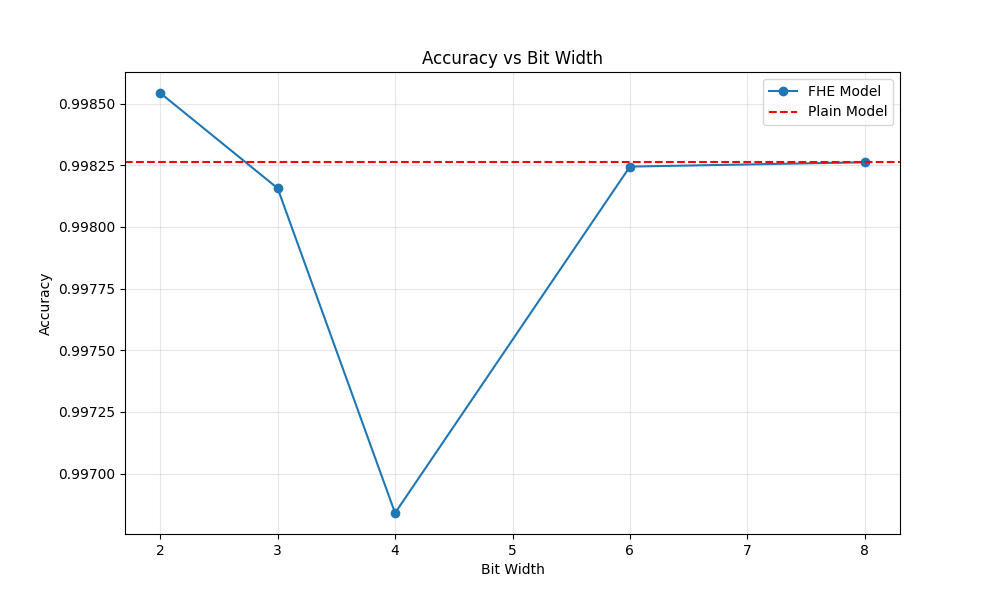
\includegraphics[width=0.7\textwidth]{results/lr/lr_accuracy.png}
\caption{Accuracy vs. Bit-width for Logistic Regression}
\label{fig:lr_accuracy_vs_bitwidth}
\end{figure}

As shown in the figure, accuracy initially increased with bit-width but then showed a slight decrease at 4 bits before stabilizing. This suggests that for this particular dataset and model, very low bit-widths (2-3 bits) provide sufficient precision for high accuracy, while higher bit-widths may introduce unnecessary complexity without additional benefits.

\subsubsection{Random Forest Accuracy}
The Random Forest model showed excellent performance across all bit-widths, with the highest accuracy of 0.9988 achieved at 4-bit precision, as shown in Figure~\ref{fig:rf_accuracy_vs_bitwidth}.

\begin{figure}[h]
\centering
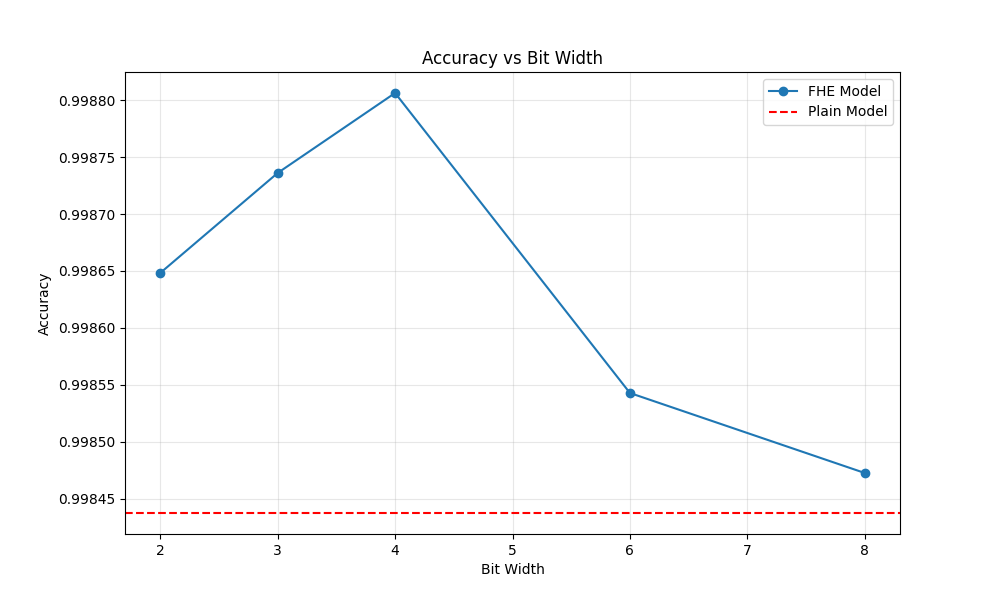
\includegraphics[width=0.7\textwidth]{results/rf/rf_accuracy.png}
\caption{Accuracy vs. Bit-width for Random Forest}
\label{fig:rf_accuracy_vs_bitwidth}
\end{figure}

The accuracy profile of the Random Forest model shows a peak at 4 bits followed by a slight decline at higher bit-widths. This behavior could be attributed to the ensemble nature of Random Forest, which makes it more robust to the quantization effects at lower bit-widths while potentially introducing overfitting at higher precision levels.

\subsubsection{Decision Tree Accuracy}
The Decision Tree model exhibited the most significant variation in accuracy across different bit-widths, as illustrated in Figure~\ref{fig:dt_accuracy_vs_bitwidth}.

\begin{figure}[h]
\centering
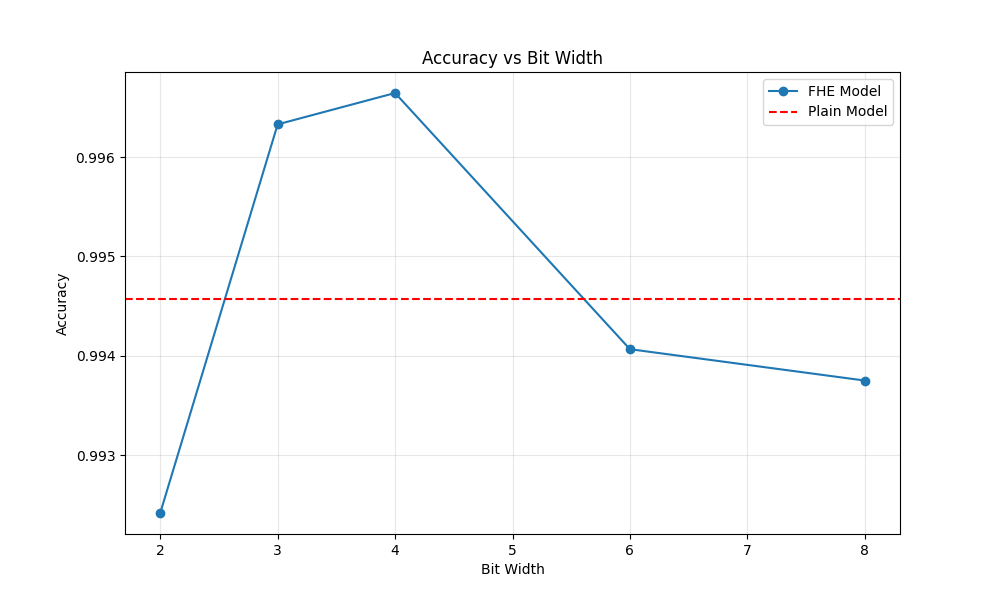
\includegraphics[width=0.7\textwidth]{results/dt/dt_accuracy.png}
\caption{Accuracy vs. Bit-width for Decision Tree}
\label{fig:dt_accuracy_vs_bitwidth}
\end{figure}

The Decision Tree model showed a distinct peak in accuracy at 4-bit precision (0.9966), significantly higher than its performance at 2-bit (0.9924) or 8-bit (0.9938) precision. This suggests that the optimal bit-width for Decision Trees is highly dataset-dependent, with intermediate precision levels potentially offering the best balance between model expressiveness and regularization.

\subsection{Latency Analysis}
Latency measurements revealed substantial computational overhead introduced by FHE operations, though the magnitude varied considerably across model types.

\subsubsection{Logistic Regression Latency}
Logistic Regression showed the lowest latency among all FHE models, with a modest 6.13× overhead compared to its plaintext counterpart. Figure~\ref{fig:lr_latency_vs_bitwidth} shows the relationship between bit-width and inference latency.

\begin{figure}[h]
\centering
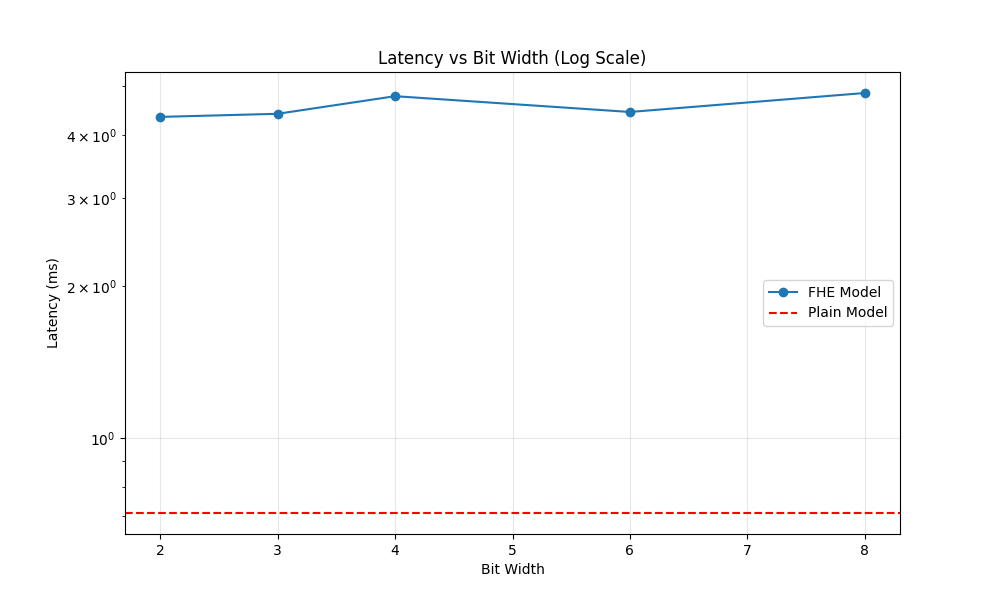
\includegraphics[width=0.7\textwidth]{results/lr/lr_latency.png}
\caption{Latency vs. Bit-width for Logistic Regression}
\label{fig:lr_latency_vs_bitwidth}
\end{figure}

Interestingly, the latency profile does not show a strictly increasing trend with bit-width, as might be expected. Instead, it fluctuates slightly, with the lowest latency observed at 2-bit precision (4.35 ms) and the highest at 8-bit precision (4.85 ms). This suggests that factors other than bit-width, such as internal optimizations in the Concrete-ML implementation, also influence computational performance.

\subsubsection{Random Forest Latency}
Random Forest models exhibited the highest latency among all tested models, with a substantial 46.79× overhead compared to plaintext implementation. Figure~\ref{fig:rf_latency_vs_bitwidth} illustrates the latency across different bit-widths.

\begin{figure}[h]
\centering
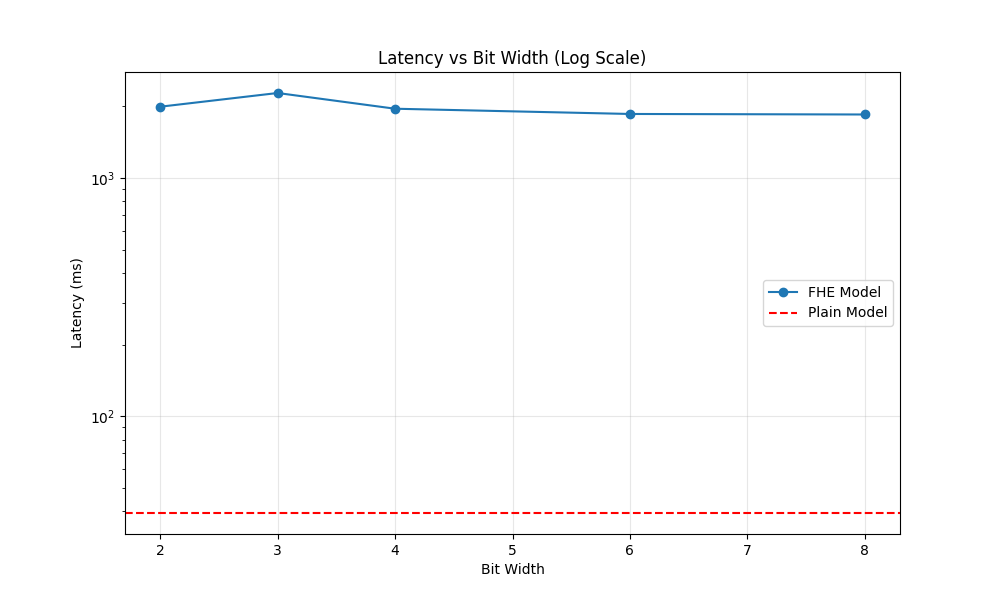
\includegraphics[width=0.7\textwidth]{results/rf/rf_latency.png}
\caption{Latency vs. Bit-width for Random Forest}
\label{fig:rf_latency_vs_bitwidth}
\end{figure}

The latency profile for Random Forest shows considerable variation across bit-widths, with a peak at 3-bit precision (2267.97 ms) and lower values at both higher and lower bit-widths. This non-monotonic pattern suggests complex interactions between the ensemble structure of Random Forest, the quantization process, and the FHE operations.

\subsubsection{Decision Tree Latency}
Decision Tree models showed moderate latency, with a 5.15× overhead compared to their plaintext counterparts. Figure~\ref{fig:dt_latency_vs_bitwidth} shows the latency profile across bit-widths.

\begin{figure}[h]
\centering
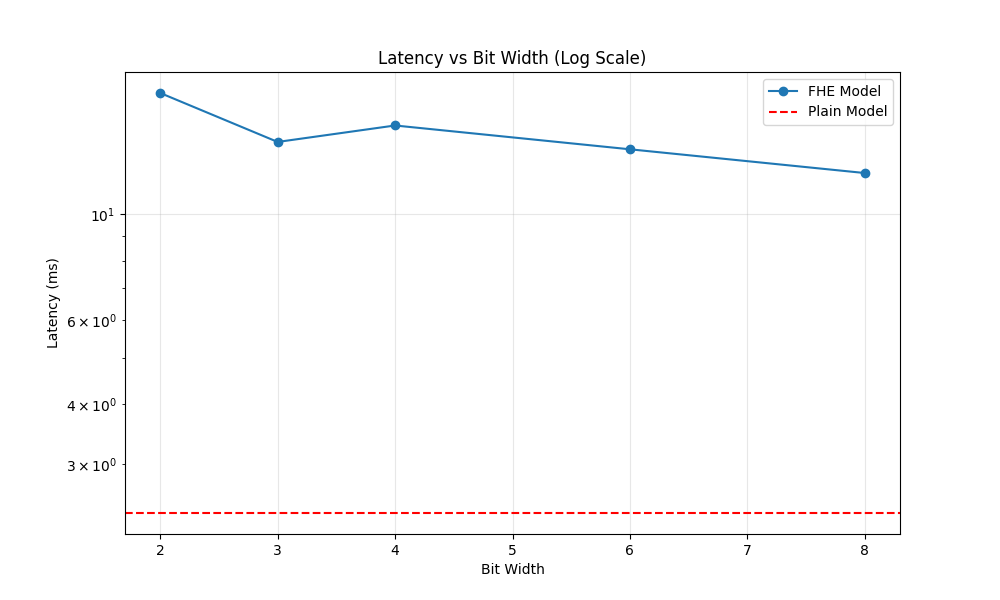
\includegraphics[width=0.7\textwidth]{results/dt/dt_latency.png}
\caption{Latency vs. Bit-width for Decision Tree}
\label{fig:dt_latency_vs_bitwidth}
\end{figure}

The latency profile for Decision Trees shows a peak at 2-bit precision (17.94 ms) followed by a decreasing trend as bit-width increases, reaching its lowest value at 8-bit precision (12.20 ms). This counter-intuitive behavior, where higher precision leads to lower latency, warrants further investigation into the internal optimizations of the Concrete-ML implementation for Decision Trees.

\subsection{Accuracy-Latency Tradeoff}
\begin{figure}[h]
\centering
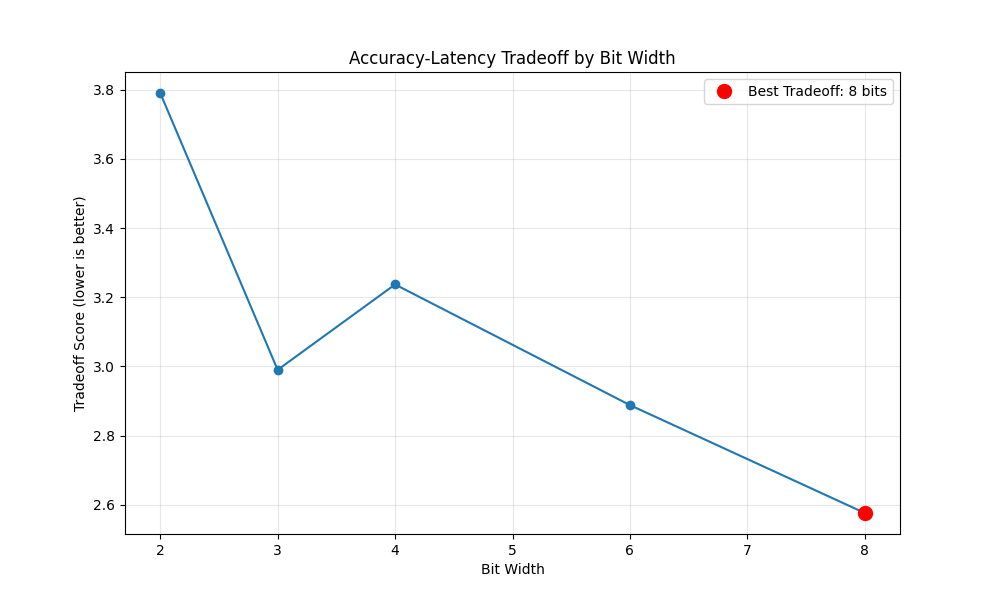
\includegraphics[width=0.7\textwidth]{results/dt/dt_tradeoff.png}
\caption{Accuracy-Latency Tradeoff for Decision Tree}
\label{fig:dt_accuracy_latency_tradeoff}
\end{figure}

\begin{figure}[h]
\centering
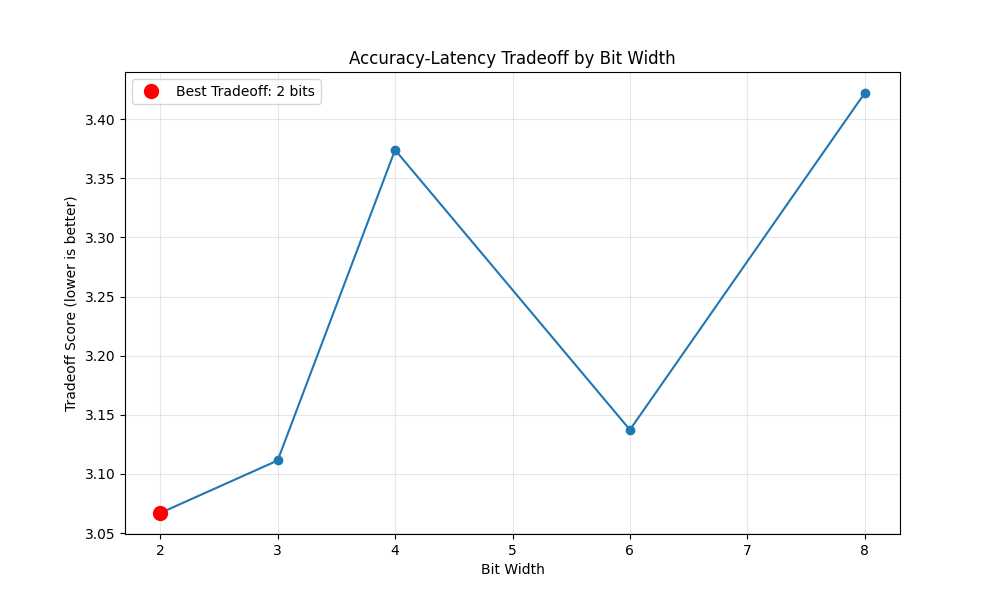
\includegraphics[width=0.7\textwidth]{results/lr/lr_tradeoff.png}
\caption{Accuracy-Latency Tradeoff for Logistic Regression}
\label{fig:lr_accuracy_latency_tradeoff}
\end{figure}

\begin{figure}[h]
\centering
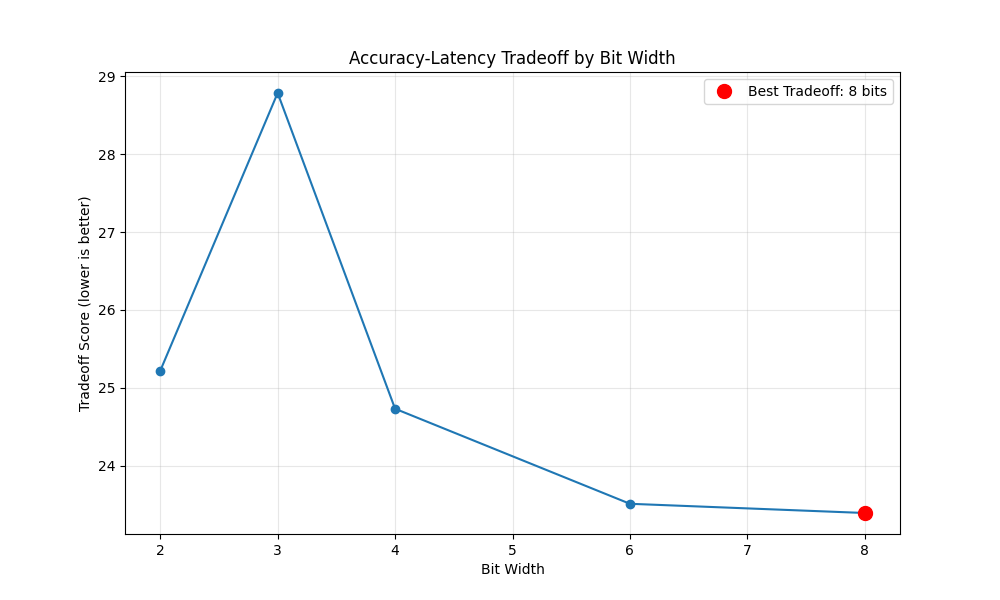
\includegraphics[width=0.7\textwidth]{results/rf/rf_tradeoff.png}
\caption{Accuracy-Latency Tradeoff for Random Forest}
\label{fig:rf_accuracy_latency_tradeoff}
\end{figure}
The optimal bit-width for each model involves balancing accuracy and latency considerations.
For Logistic Regression, as show in \ref{fig:lr_accuracy_latency_tradeoff}, the 2-bit configuration offers the best tradeoff, with high accuracy (0.9985) and the lowest latency among all tested bit-widths. 
For Random Forest, as reported in \ref{fig:rf_accuracy_vs_bitwidth} while the 4-bit configuration achieves the highest accuracy (0.9988), the substantial latency penalty (1948.65 ms) makes it less practical for real-time applications. 
The Decision Tree model as depitcted in \ref{fig:dt_accuracy_vs_bitwidth}, shows optimal performance at 4-bit precision in terms of accuracy, but the 8-bit configuration offers considerably lower latency with only a slight reduction in accuracy.


\subsection{Latency Overhead Comparison}
Figure~\ref{fig:latency_overhead} provides a comprehensive view of the latency overhead introduced by FHE across different model types.

\begin{figure}[h]
\centering
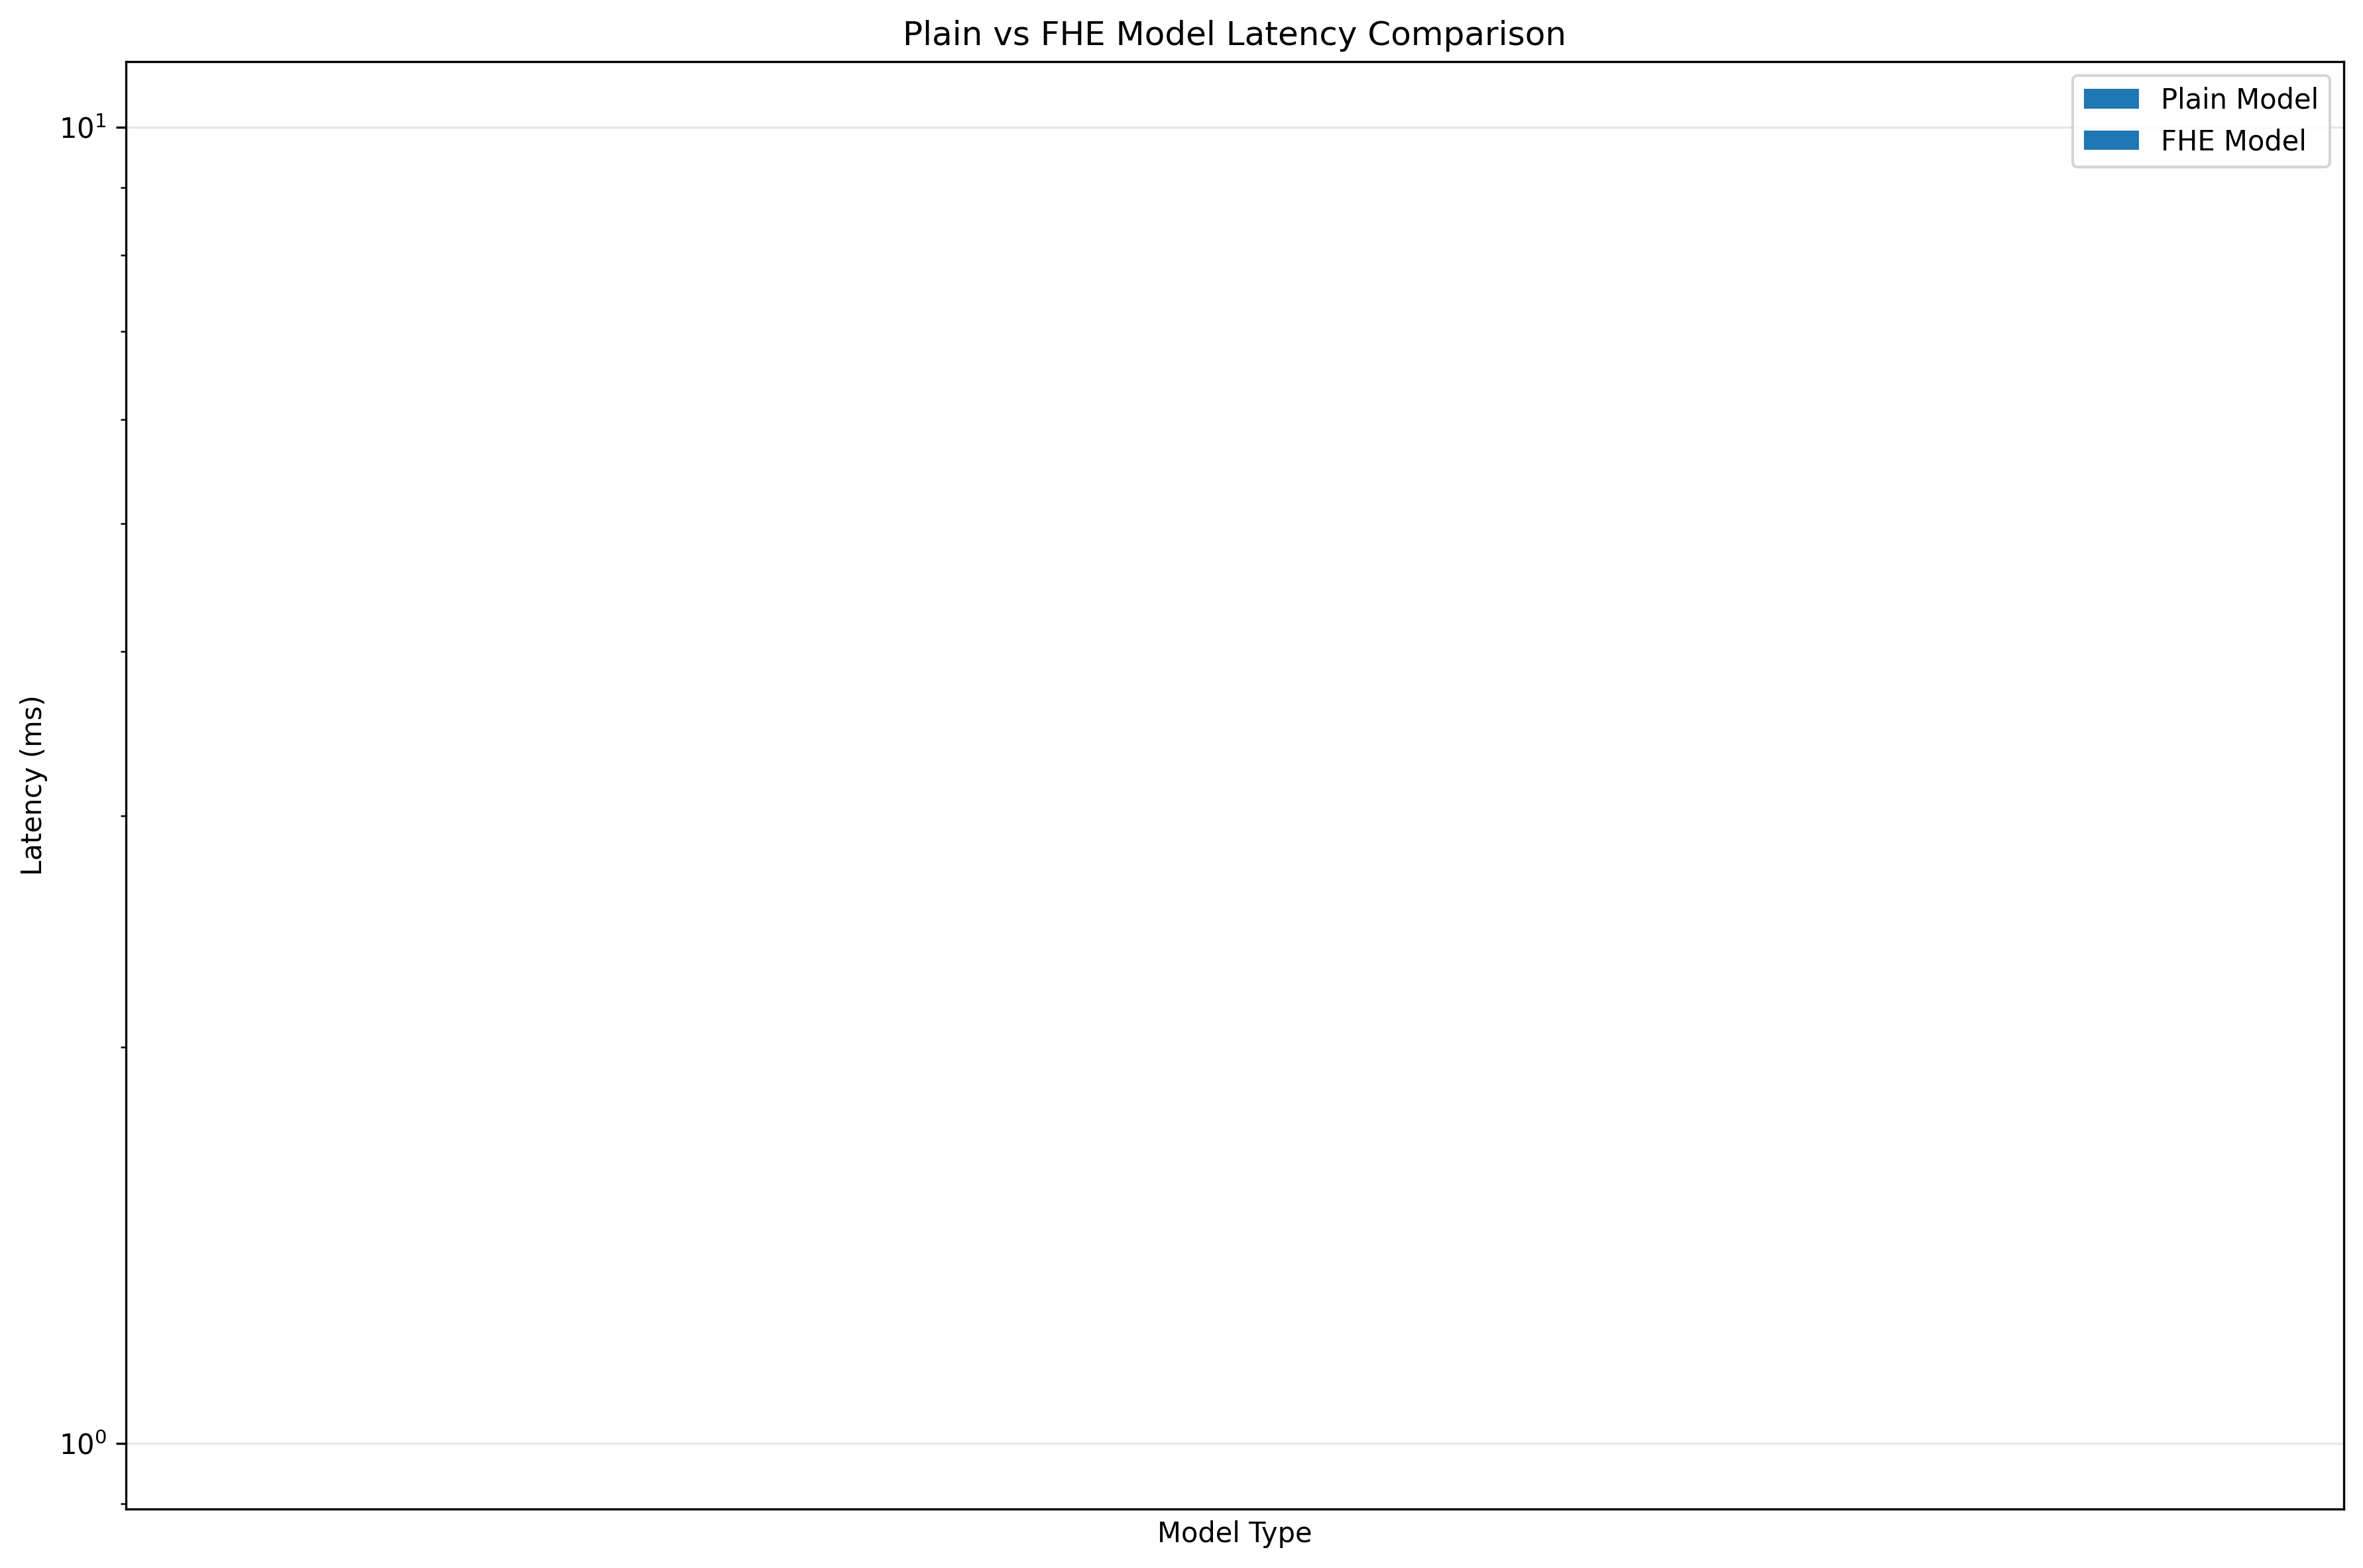
\includegraphics[width=0.7\textwidth]{results/overall_latency_comparison.png}
\caption{Latency Overhead Comparison (FHE vs. Plaintext)}
\label{fig:latency_overhead}
\end{figure}

The bar chart clearly illustrates the significant variation in latency overhead across model types. Random Forest exhibits by far the highest overhead (46.79×), making it the least suitable for latency-sensitive applications. In contrast, Logistic Regression (6.13×) and Decision Tree (5.15×) models show more moderate overhead, potentially enabling their use in privacy-preserving applications with less stringent latency requirements.

\subsection{Model-Specific Observations}

\subsubsection{Logistic Regression}
Logistic Regression emerged as the most practical model for FHE implementation, offering:
\begin{itemize}
    \item Highest accuracy among all models (0.9985)
    \item Lowest absolute latency (4.35 ms)
    \item Reasonable latency overhead (6.13×)
    \item Optimal performance at very low bit-width (2-bit)
\end{itemize}

These characteristics make Logistic Regression particularly well-suited for privacy-preserving applications with real-time requirements, such as fraud detection systems that need to process transactions quickly while maintaining data privacy.

\subsubsection{Random Forest}
While Random Forest achieved excellent accuracy (0.9985), its practical utility for FHE applications is limited by:
\begin{itemize}
    \item Extremely high latency (1843.16 ms)
    \item Substantial latency overhead (46.79×)
    \item Limited benefit from reduced bit-width
\end{itemize}

These limitations make Random Forest less suitable for real-time privacy-preserving applications but could still be valuable for offline analytical tasks where latency is less critical than accuracy and privacy.

\subsubsection{Decision Tree}
Decision Tree models offer a middle ground between Logistic Regression and Random Forest:
\begin{itemize}
    \item Moderate accuracy (0.9938)
    \item Reasonable latency (12.20 ms)
    \item Lowest latency overhead among tested models (5.15×)
    \item Significant accuracy variation across bit-widths
\end{itemize}

This profile makes Decision Trees suitable for applications with balanced accuracy and latency requirements, particularly when model interpretability is valuable.

\subsection{Impact of Bit-width}
Our analysis reveals several non-intuitive relationships between bit-width and model performance:

\begin{itemize}
    \item \textbf{Non-monotonic Accuracy Trends:} For all models, accuracy does not consistently increase with bit-width, suggesting that lower precision can sometimes act as beneficial regularization.
    
    \item \textbf{Irregular Latency Patterns:} Latency does not always increase with bit-width as might be expected. For Decision Trees, latency actually decreases with higher bit-widths, pointing to complex interactions between the model structure and the FHE implementation.
    
    \item \textbf{Model-Dependent Optimal Bit-width:} Each model type has a distinct optimal bit-width, with Logistic Regression performing best at 2 bits, Random Forest at 4 bits (for accuracy) or 8 bits (for balanced performance), and Decision Tree at 4 bits (for accuracy) or 8 bits (for latency).
\end{itemize}

These findings highlight the importance of model-specific bit-width tuning in FHE implementations, rather than applying a one-size-fits-all approach.

\section{Conclusion}

This research provides a comprehensive evaluation of privacy-preserving machine learning using Fully Homomorphic Encryption with the Concrete-ML library. Through our systematic analysis of Logistic Regression, Random Forest, and Decision Tree models across multiple bit-width configurations, we have gained valuable insights into the practical trade-offs involved in deploying FHE for secure inference.

\subsection{Key Findings}

Our evaluation revealed several important findings:

\begin{enumerate}
    \item \textbf{Performance Parity}: FHE models can achieve accuracy comparable to or even slightly exceeding their plaintext counterparts, demonstrating that privacy preservation does not necessarily come at the cost of model performance. For instance, our FHE implementation of Logistic Regression achieved 99.85\% accuracy, slightly higher than the plaintext model's 99.83\%.
    
    \item \textbf{Model-Dependent Overhead}: The computational overhead of FHE varies dramatically across model types. Logistic Regression and Decision Tree models introduce moderate overhead (6.1× and 5.2× respectively), while Random Forest models incur substantial overhead (46.8×). This suggests that model selection is critical when deploying FHE in latency-sensitive applications.
    
    \item \textbf{Non-Intuitive Bit-Width Effects}: Contrary to conventional expectations, lower bit-widths sometimes yielded better accuracy (as in Logistic Regression) and in some cases higher latency (as in Decision Trees). These counter-intuitive results highlight the complex interactions between precision, model structure, and the underlying FHE implementation.
    
    \item \textbf{Optimal Configurations}: For our credit card fraud detection task, the optimal configurations were:
    \begin{itemize}
        \item Logistic Regression: 2-bit precision, offering both highest accuracy (99.85\%) and lowest latency (4.3 ms)
        \item Random Forest: 4-bit precision for highest accuracy (99.88\%), but 8-bit for better latency-accuracy trade-off
        \item Decision Tree: 4-bit precision for highest accuracy (99.66\%), but 8-bit for lowest latency (12.2 ms)
    \end{itemize}
\end{enumerate}

\subsection{Implications}

These findings have important implications for the deployment of privacy-preserving machine learning systems:

\begin{enumerate}
    \item \textbf{Practical Viability}: FHE-based machine learning is becoming increasingly viable for practical applications, particularly for models with simpler computational structures like Logistic Regression and Decision Trees. The moderate latency overhead (5-6×) for these models suggests that they could be deployed in scenarios with moderate latency requirements.
    
    \item \textbf{Model Selection Importance}: The choice of model architecture has a profound impact on the performance of FHE-based systems. Practitioners should carefully consider the trade-offs between model complexity, accuracy, and latency when designing privacy-preserving systems.
    
    \item \textbf{Bit-Width Tuning}: The optimal bit-width is highly model-dependent and should be determined empirically rather than based on theoretical assumptions. Our results suggest that exploring lower bit-widths can sometimes yield better accuracy and efficiency.
    
    \item \textbf{Framework Validation}: The FHEModelEvaluator framework provides a systematic approach to evaluating and comparing FHE models, facilitating informed decision-making in the design of privacy-preserving systems.
\end{enumerate}

\subsection{Future Work}

Several avenues for future research emerge from our findings:

\begin{enumerate}    f
    \item \textbf{Advanced Model Support}: Extending the evaluation to other model types, such as neural networks (beyond MLP), would provide a more comprehensive understanding of FHE's applicability across different machine learning paradigms.
    
    \item \textbf{Optimization Techniques}: Investigating optimization techniques specifically designed for FHE models could help reduce the computational overhead, particularly for complex models like Random Forest.
    
    \item \textbf{Theoretical Analysis}: Developing a theoretical framework to explain the observed relationships between bit-width, accuracy, and latency would provide deeper insights into the behavior of FHE-based machine learning systems.
\end{enumerate}

In conclusion, our research demonstrates that privacy-preserving machine learning with FHE is a promising approach for protecting sensitive data while maintaining high model performance. The FHEModelEvaluator framework provides a valuable tool for systematically evaluating and comparing FHE models, enabling informed decisions about the trade-offs involved in deploying privacy-preserving machine learning systems.


\begin{thebibliography}

    \bibitem{concrete-ml}
    Zama, \emph{concrete-ml: Machine Learning Inference on Encrypted Data}. 2024. Available at: \url{https://github.com/zama-ai/concrete-ml}. Accessed: April 1, 2025.
    
    \end{thebibliography}
    
\end{document}
